\documentclass{beamer}
\usetheme[white]{Wisconsin}
\usepackage{wrapfig}
\usepackage{longtable}
\usepackage{listings}
\usepackage{color}
%% The amssymb package provides various useful mathematical symbols
\usepackage{amssymb}
%% The amsthm package provides extended theorem environments
\usepackage{amsthm} \usepackage{amsmath}
\usepackage[mathcal]{euscript} \usepackage{color}
\usepackage{textcomp}
\usepackage{algorithm,algorithmic}
\usepackage[absolute,overlay]{textpos}
  \setlength{\TPHorizModule}{1mm}
  \setlength{\TPVertModule}{1mm}
\definecolor{listinggray}{gray}{0.9}
\definecolor{lbcolor}{rgb}{0.9,0.9,0.9}
\lstset{
  backgroundcolor=\color{lbcolor},
  tabsize=4,
  rulecolor=,
  language=c++,
  basicstyle=\scriptsize,
  upquote=true,
  aboveskip={1.5\baselineskip},
  columns=fixed,
  showstringspaces=false,
  extendedchars=true,
  breaklines=true,
  prebreak =
  \raisebox{0ex}[0ex][0ex]{\ensuremath{\hookleftarrow}},
  frame=single,
  showtabs=false,
  showspaces=false,
  showstringspaces=false,
  identifierstyle=\ttfamily,
  keywordstyle=\color[rgb]{0,0,1},
  commentstyle=\color[rgb]{0.133,0.545,0.133},
  stringstyle=\color[rgb]{0.627,0.126,0.941},
}
\AtBeginSection[]
{
  \begin{frame}<beamer>
    \frametitle{Outline}
    \tableofcontents[currentsection]
  \end{frame}
}

%% colors
\setbeamercolor{boxheadcolor}{fg=white,bg=UWRed}
\setbeamercolor{boxbodycolor}{fg=black,bg=white}

\setbeamerfont{block body}{size=\footnotesize}

%%----------------------------------------------------------------------------%%
\author{Alex P. Robinson
    \\ Engineering Physics Department
    \\ University of Wisconsin - Madison
    \\ Preliminary Examination
}

\date{\today}
\title{Development of a Monte Carlo Code System with Continuous Energy Adjoint Transport Capabilities for Neutrons and Photons} 
\begin{document}
\maketitle
%%----------------------------------------------------------------------------%%
%% Overview
%%----------------------------------------------------------------------------%%
\begin{frame}{Outline}

  \tableofcontents

\end{frame}

%%----------------------------------------------------------------------------%%
\section{Introduction}
%%----------------------------------------------------------------------------%%
\subsection{The Monte Carlo Method}
%%----------------------------------------------------------------------------%%
\begin{frame}{The Monte Carlo method}

  \begin{itemize}
    \item The Monte Carlo method is a stochastic method in which samples are
      drawn from a parent population through sampling procedures governed by
      a set of probability laws.
      \medskip
    \item From the samples, statistical data is acquired and analyzed to make
      inferences about the parent population.
  \end{itemize}
  
  \medskip
  \medskip
  
  \begin{beamerboxesrounded}[upper=boxheadcolor,lower=boxbodycolor,shadow=true]{Radiation Transport Problems}
    \begin{itemize}
      \item \textbf{System of Interest:} collection of bounded regions 
        containing a material, vacuum, source or detector
      \item \textbf{Parent Population:} set of all possible radiation histories
      \item \textbf{Sample:} radiation history drawn from set of all possible 
        histories
      \item \textbf{Probability Laws:} related to material interaction cross 
        sections
      \item \textbf{Sampling Process Variations}: forward and adjoint
    \end{itemize}
  \end{beamerboxesrounded}
    
\end{frame}

%%----------------------------------------------------------------------------%%
\begin{frame}{The Forward Process vs. the Adjoint Process}

  \medskip

  \begin{beamerboxesrounded}[upper=boxheadcolor,lower=boxbodycolor,shadow=true]{The Forward Process}
    \begin{itemize}
      \item Starting point of a history is sampled from the source
      \item Information about the history is recorded in the detector
      \item Probability laws used for sampling states of the history
        can be derived from the \textit{transport equation}
    \end{itemize}
  \end{beamerboxesrounded}

  \bigskip
  \medskip

  \begin{beamerboxesrounded}[upper=boxheadcolor,lower=boxbodycolor,shadow=true]{The Adjoint Process}
    \begin{itemize}
      \item Starting point of a history is sampled from the detector
      \item Information about the history is recorded in the source
      \item Probability laws used for sampling states of the history
        can be derived from the \textit{adjoint transport equation}
    \end{itemize}
  \end{beamerboxesrounded}

\end{frame}

%%----------------------------------------------------------------------------%%
\subsection{Motivations for using the adjoint process}
%%----------------------------------------------------------------------------%%
\begin{frame}{Motivations for Using the Adjoint Process}

  \begin{enumerate}
    \item Motivation 1: The source and detector phase space
      \smallskip
      \begin{itemize}
        \item Adjoint process generally more efficient than forward process 
          when phase space of source is larger than phase space of detector
      \end{itemize}
      \bigskip
      \bigskip
    \item Motivation 2: The adjoint flux interpretation
      \smallskip
      \begin{itemize}
        \item Adjoint process estimates a quantity called the adjoint flux
          \medskip
        \item Physical interpretation of the adjoint flux is a source 
          importance or sensitivity to the detector response
          \medskip
        \item Adjoint flux can be invaluable when exact source 
          distribution is not known (optimization problems)
      \end{itemize}
  \end{enumerate}

  \bigskip

  \begin{itemize}
    \item Three classes of problems will be discussed that can benefit from
      the adjoint process
  \end{itemize}

\end{frame}

%%----------------------------------------------------------------------------%%
\begin{frame}{Shutdown Dose Calculations Using the R2S(A) Method}

  \begin{itemize}
    \item Photon dose in a region of a nuclear system resulting from neutron 
      activation of material is desired
      \medskip
    \item This information is useful for planning maintenance on the system
      \medskip
    \item These problems are often solved using the rigorous 2-step method (R2S)
      \medskip
    \item The adjoint process can be useful for small regions of interest
  \end{itemize}

  \medskip
  \medskip

  \begin{beamerboxesrounded}[upper=boxheadcolor,lower=boxbodycolor,shadow=true]
    {The R2S(A) method}
    \begin{enumerate}
      \item Neutron flux throughout the system is calculated
        \smallskip
      \item Activation code calculates the material activation and photon
        sources from neutron flux data
        \smallskip
      \item Photon dose calculated in areas of interest using a forward
        process or an adjoint process (A)
    \end{enumerate}
  \end{beamerboxesrounded}

\end{frame}

%%----------------------------------------------------------------------------%%
%% \begin{frame}{Shutdown Dose Calculations Using the R2SA Method}
  
%%   \begin{itemize}
%%     \item Amount of activated material is often much larger than the region 
%%       where the dose distribution is desired 
%%       \medskip
%%     \item These problems could potentially benefit from the adjoint process
%%       for photons
%%       \medskip
%%     \item When the adjoint process is used, the solution method is called the
%%       rigorous 2-step adjoint method (R2SA)
%%   \end{itemize}

%%   \medskip
%%   \medskip

%%   \begin{beamerboxesrounded}[upper=boxheadcolor,lower=boxbodycolor,shadow=true]{The R2SA method}
%%     \begin{enumerate}
%%       \item Neutron flux throughout the experiment or device is calculated
%%         \smallskip
%%       \item Activation code calculates the material activation and photon
%%         sources from the neutron flux data
%%         \smallskip
%%       \item Photon dose is calculated in areas of interest using an adjoint
%%         process 
%%     \end{enumerate}
%%   \end{beamerboxesrounded}

%% \end{frame}

%%----------------------------------------------------------------------------%%
\begin{frame}{Permanent Implant Brachytherapy}

  \begin{textblock}{120}(4,15)
    \begin{itemize}
      \item \textbf{Optimization goal:} determine a source configuration
        that provides an optimal dose distribution to the target while
        minimizing the dose to sensitive structures
        \medskip
      \item Adjoint flux data allows one to eliminate source positions that 
        result in a high dose to sensitive structures relative to the target
        \smallskip
        \begin{itemize}
          \item Shown to simplify and speed up optimization algorithms
        \end{itemize}
    \end{itemize}
  \end{textblock}

   \begin{textblock}{20}(2,50)
    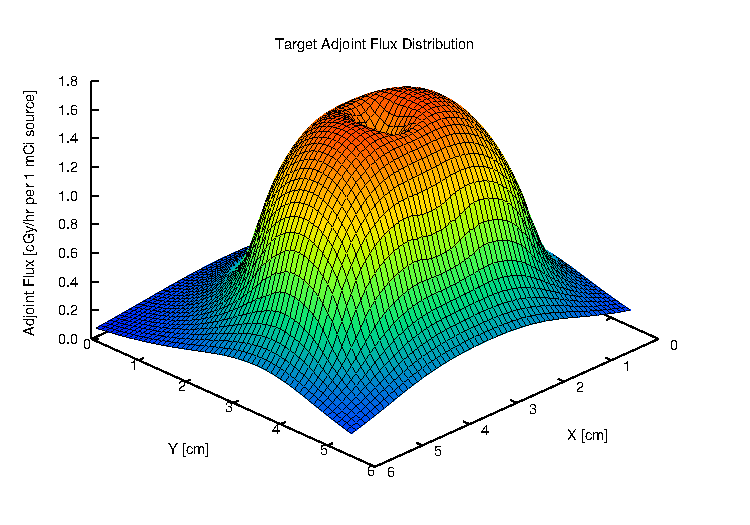
\includegraphics[width=2.5in]{figures/Target_adjoint_flux-midplane.pdf}
  \end{textblock}

   \begin{textblock}{20}(65,50)
    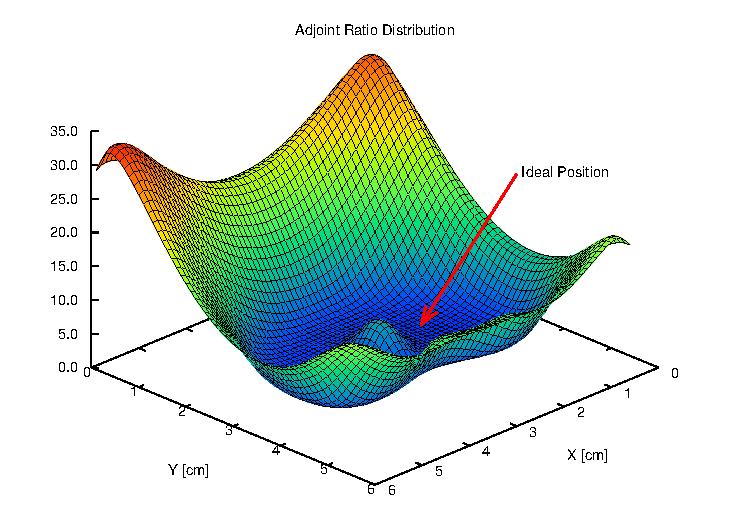
\includegraphics[width=2.5in]{figures/adjoint_ratio-slice5.pdf}
  \end{textblock}

\end{frame}

%%----------------------------------------------------------------------------%%
\begin{frame}{Detector Design}
  
  \begin{textblock}{120}(4,15)
    \begin{itemize}
      \item Adjoint flux can allow for spectral performance of a detector to be 
        predicted for an arbitrary source distribution
        \medskip
      \item Detector design can then be optimized before it is constructed
        \smallskip
        \begin{itemize}
          \item Important for detectors with rare materials (e.g. $He^3$ 
            neutron detectors)
        \end{itemize}
    \end{itemize}
  \end{textblock}

  \begin{textblock}{20}(2,45)
    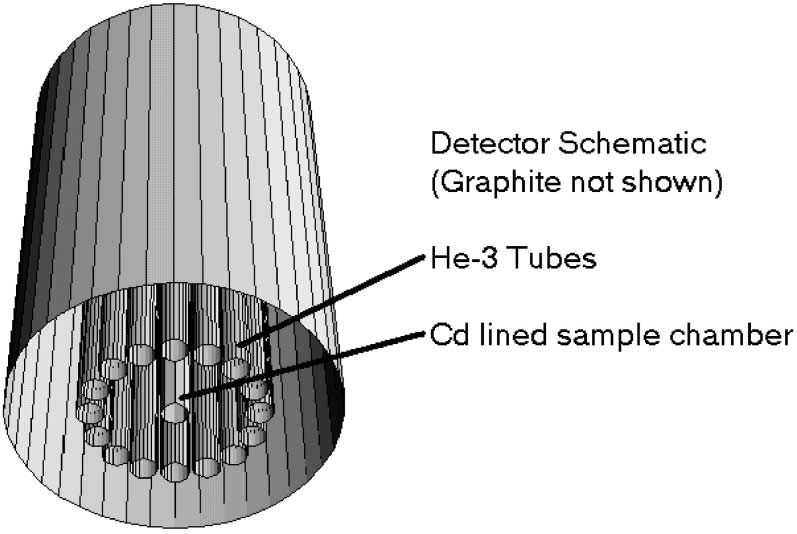
\includegraphics[width=2.5in]{figures/He3_detector.png}
  \end{textblock}

  \begin{textblock}{20}(70,49)
    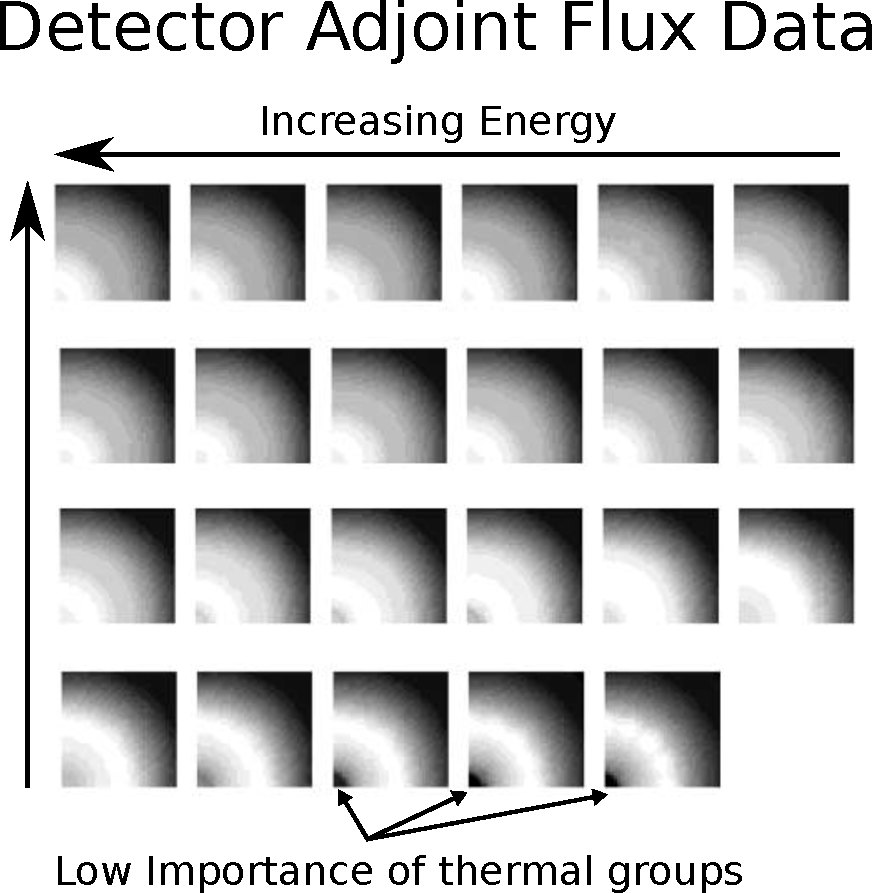
\includegraphics[width=1.8in]{figures/He3_detector_adjoint_data_modified.pdf}
  \end{textblock}

  \begin{textblock}{50}(4,90)
    (Sjoden, 2002)
  \end{textblock}

\end{frame}

%%----------------------------------------------------------------------------%%
\subsection{Monte Carlo codes available today}
%%----------------------------------------------------------------------------%%
\begin{frame}{Continuous Energy Capabilities of Popular Codes}
  
  \begin{table}[ht]
    \centering
    \begin{tabular}{c c c c c }
      \hline\hline
      Code & $n$ & $\gamma$ &  $n^{\dagger}$ & $\gamma^{\dagger}$ \\ [0.5ex]
      \hline
      EGS4 & - & $\surd$ & - & - \\
      EGSnrc & - & $\surd$ & - & - \\
      ITS6 & - & $\surd$ & - & - \\
      PENELOPE & - & $\surd$ & - & - \\
      MORSE & - & - & - & - \\
      TART2005 & $\surd$ & $\surd$ & - & - \\
      MCNP5/6 & $\surd$ & $\surd$ & - & - \\
      MCNPX & $\surd$ & $\surd$ & - & - \\
      GEANT4 & $\surd$ & $\surd$ & - & $\surd$ \\
      MCBEND & $\surd$ & $\surd$ & $\surd$ & - \\ [1ex]
      \hline
      FACEMC & $\surd$ & $\surd$ & $\surd$ & $\surd$ \\ [1ex]
      \hline
    \end{tabular}
  \end{table}

\begin{itemize}
  \item A lack of necessary adjoint cross section data is a major deterrent to
    implementing the adjoint process on a continuous energy scale.
\end{itemize}
  
\end{frame}

%%----------------------------------------------------------------------------%%
\section{The Monte Carlo Random Walk Process}
%%----------------------------------------------------------------------------%%
\subsection{General Monte Carlo theory}
%%----------------------------------------------------------------------------%%
\begin{frame}{Fredholm Integral Equations of the Second Kind (FIESKs)}
  
  \begin{equation*}
    F(x) = S(x) + \lambda \int_a^b K(x,y) F(y)dy
  \end{equation*}

  \bigskip
  
  \begin{itemize}
    \item Important equation for radiation transport 
      \medskip
    \item $S(x)$ is a forcing function
      \medskip
    \item $K(x,y)$ is the kernel of the integral equation
      \begin{itemize}
        \smallskip
        \item Characterizes the transition from some initial state y to
          the state x
          \smallskip
        \item Often written as $K(y \to x)$ to signify this interpretation
      \end{itemize}
  \end{itemize}
  
\end{frame}

%%----------------------------------------------------------------------------%%
\begin{frame}{Volterra Integral Equations of the Second Kind}

  \begin{equation*}
    F(x) = S(x) + \lambda \int_a^x K(y \to x) F(y) dy
  \end{equation*}

  \bigskip
  
  \begin{itemize}
    \item Very similar to the FIESK except one limit of integration is variable
      \medskip
    \item Comes about whenever there is a preferred direction for the 
      independent variable (i.e. particle scattering kinematics)
      \medskip
    \item Can be converted to a FIESK using a modified kernel
  \end{itemize}

  \begin{equation*}
    F(x) = S(x) + \lambda \int_a^b K^{'}(y \to x) F(y) dy \nonumber
  \end{equation*}
  
  \begin{equation*}
    K^{'}(y \to x) = 
    \begin{cases}
      K(y \to x) & \text{if }y < x \\
      0 & \text{if }y > x.
    \end{cases}
  \end{equation*}

\end{frame}

%%----------------------------------------------------------------------------%%
\begin{frame}{The Method of Successive Approximations}

  \begin{align}
    f_0(x) & = S(x) \nonumber \\
    f_n(x) & = S(x) + \lambda \int_a^b K(y \to x)f_{n-1}(y)dy \nonumber \\
    & \quad \nonumber \\
    F(x) & = \lim_{n \to \infty} f_n(x) \nonumber
  \end{align}

  \begin{itemize}
    \item The solution is more commonly expressed as a Neumann series:
  \end{itemize}
  \begin{align}
    F(x) & = S(x) + \lambda \int_a^b K(y \to x)S(y)dy \text{ }+ \nonumber \\
    & \quad \lambda^2 \int_a^b \int_a^b K(y \to x)K(y_1 \to y)S(y_1)dy_1dy 
    \text{ } + \nonumber \\
    & \quad \lambda^3 \int_a^b \int_a^b \int_a^b K(y \to x)K(y_1 \to y)
    K(y_2 \to y_1)S(y_2)dy_2dy_1dy \text{ }+ \nonumber \\
    & \quad \cdots \nonumber
  \end{align}
  
\end{frame}

%%----------------------------------------------------------------------------%%
\begin{frame}{The Monte Carlo Method}

  \begin{equation*}
    \text{Random Walk: }
    \begin{cases}
      p^1(x) & = \frac{S(x)}{\int S(x)dx} \\ 
      p(y \to x) & = C(y)K(y \to x)  \\
      p(y) & = 1 - \int_a^b p(y \to x) dx.
    \end{cases}
    \label{eq:mc_random_walk_pdfs}
  \end{equation*}

  \bigskip

  \begin{itemize}
    \item $p^1(x)$ represents the probability of a random walk starting in
      state $x$
      \medskip
    \item $p(y \to x)$ characterizes the probability of a transition from
      initial state $y$ to new state $x$
      \medskip
    \item $p(y)$ represents the probability of termination in state $y$
      \medskip
    \item From these probability distribution functions (PDFs) random walks
      can be constructed
      \medskip
    \item Using special statistical rules, called estimators, the solution to
      the FIESK can be estimated from the random walks
  \end{itemize}

\end{frame}

%%----------------------------------------------------------------------------%%
%% \begin{frame}{Proof That the Monte Carlo Method Recovers the Solution}

%%   \begin{itemize}
%%     \item First define the event density as the expected value of the number
%%       density of events that happen in state $x$:
%%       \begin{align}
%%         P(x) = 1 \cdot &P^1(x) + 1 \cdot P^2(x) + \ldots 
%%         = \sum_{n=1}^{\infty} P^n(x) \nonumber \\
%%         P^1(x) & = p^1(x) \nonumber \\
%%         P^n(x) & = \int_{\Gamma} p(y \to x) P^{n-1}(y)dy. \nonumber
%%       \end{align}
%%     \item Using the event density and the Monte Carlo method, the solution
%%       to a FIESK is recovered:
%%       \begin{align}
%%         P(x) & = \sum_{n=1}^{\infty} P^n(x) \nonumber
%%         = p^1(x) + \int_{\Gamma} p(y \to x) \sum_{n=2}^{\infty} P^{n-1}(y)dy 
%%         \nonumber\\
%%         & = p^1(x) + \int_{\Gamma} p(y \to x) P(y)dy \nonumber.
%%       \end{align}
%%   \end{itemize}

%% \end{frame}

%%----------------------------------------------------------------------------%%
\subsection{The Monte Carlo random walk process for radiation transport}
%%----------------------------------------------------------------------------%%
\begin{frame}{The Transport Equation}

\begin{align}
  \hat{\Omega} \cdot \vec{\bigtriangledown} \varphi(\vec{r},E,\hat{\Omega})
    &\text{ }+\text{ } \Sigma_T(\vec{r},E) \varphi(\vec{r},E,\hat{\Omega}) = 
    S(\vec{r},E,\hat{\Omega}) \text{ }+\text{ } \nonumber \\
    & \int\int \Sigma_T(\vec{r},E^{'} \to E,\hat{\Omega}^{'} \to \hat{\Omega})
    \varphi(\vec{r},E^{'},\hat{\Omega}^{'}) dE^{'}d\hat{\Omega}^{'} \nonumber
\end{align}

  \begin{itemize}
    \item The transport equation describes the expected behavior of particles
      in a medium
      \medskip
    \item The right side of this equation is called the emission density 
      $\chi(\vec{r},E,\hat{\Omega})$
  \end{itemize}
  \medskip
  \begin{equation*}
    \chi(\vec{r},E,\hat{\Omega}) = S(\vec{r},E,\hat{\Omega}) +
    \int\int \Sigma_T(\vec{r},E^{'} \to E,\hat{\Omega}^{'} \to \hat{\Omega})
    \varphi(\vec{r},E^{'},\hat{\Omega}^{'}) dE^{'}d\hat{\Omega}^{'}
  \end{equation*}
  
  \begin{itemize}
    \item The transport equation must be converted to a FIESK to derive a 
      Monte Carlo random walk process for radiation transport
  \end{itemize}

\end{frame}

%%----------------------------------------------------------------------------%%
%% \begin{frame}{Converting the Transport Equation to an Integral Form}

%%   \begin{itemize}
%%     \item The method of characteristics will be used to convert the 
%%       transport equation to an integral form: \newline
%%       \begin{equation*}
%%         \vec{r}^{'} = \vec{r} - R\hat{\Omega}.
%%         \label{eq:characteristic}
%%       \end{equation*}
%%     \item A directional derivative along the characteristic can be determined:
%%       \newline
%%       \begin{align}
%%         \frac{d}{dR} & = \frac{dx^{'}}{dR}\frac{\partial}{\partial x} +
%%         \frac{dy^{'}}{dR}\frac{\partial}{\partial y} +
%%         \frac{dz^{'}}{dR}\frac{\partial}{\partial z} \nonumber \\
%%         & = -\Omega_x \frac{\partial}{\partial x} -
%%         \Omega_y \frac{\partial}{\partial y} -
%%         \Omega_z \frac{\partial}{\partial z} \nonumber \\
%%         & = -\hat{\Omega} \cdot \vec{\bigtriangledown}. \nonumber
%%       \end{align}
%%     \item The transport equation becomes
%%       \begin{equation*}
%%         -\frac{d}{dR}\varphi(\vec{r}^{'},E,\hat{\Omega}) + \Sigma_T(\vec{r}^{'},E)
%%         \varphi(\vec{r}^{'},E,\hat{\Omega}) =
%%         \chi(\vec{r}^{'},E,\hat{\Omega}).
%%         \label{eq:transport_ode}
%%       \end{equation*}
%%   \end{itemize}

%% \end{frame}

%%----------------------------------------------------------------------------%%
\begin{frame}{The Transport Equation in Integral Form}

  %% \begin{itemize}
  %%   \item Using the following integrating factor, the transport equation can
  %%     be converted to an integral form: \newline
  %%     \begin{equation*}
  %%       \exp{\left[-\int_0^R \Sigma_T(\vec{r}-R^{'}\hat{\Omega},E)dR^{'} \right]}.
  %%     \end{equation*}
  %%   \item By integrating the equation from 0 to $\infty$ and assuming that the
  %%     flux goes to zero as $R$ goes to $\infty$, the integral equation is
  %%     obtained:
  %% \end{itemize}

  \begin{itemize}
    \item The method of characteristics is used to convert the transport 
      equation to an ordinary differential equation (ODE)
      \medskip
    \item Subsequent solution of this ODE results in the integral transport 
      equation
  \end{itemize}
  \begin{align}
    \varphi(\vec{r},E,\hat{\Omega}) & = 
    \int_0^{\infty} \chi(\vec{r} - R\hat{\Omega},E,\hat{\Omega})
    \exp{\left[-\int_0^R \Sigma_T(\vec{r}-R^{'}\hat{\Omega},E)dR^{'} \right]} 
    dR \nonumber \\
    & = \int \chi(\vec{r}^{'},E,\hat{\Omega}) 
    \tau(\vec{r}^{'},\vec{r},E,\hat{\Omega}) dV^{'}. \nonumber
  \end{align}
  
  \begin{itemize}
    \item The function $\tau(\vec{r}^{'},\vec{r},E,\hat{\Omega})$ allows
      the line integral to be expressed as a volume integral
  \end{itemize}
  \begin{equation*}
    \tau(\vec{r}^{'},\vec{r},E,\hat{\Omega})= 
    \exp{\left[-\int_0^{|\vec{r} - \vec{r}^{'}|} 
        \Sigma_T(\vec{r}-R^{'}\hat{\Omega},E)dR^{'} \right]} 
    \frac{\delta \left(\hat{\Omega} - \left[\frac{\vec{r} - \vec{r}^{'}}
        {|\vec{r} - \vec{r}^{'}|}\right]\right)}
         {|\vec{r} - \vec{r}^{'}|^2}
  \end{equation*}

\end{frame}

%%----------------------------------------------------------------------------%%
\begin{frame}{The Emission Density FIESK}

  \begin{itemize}
    \item To construct the emission density FIESK, the integral transport 
      equation is substituted into the equation for the emission density
  \end{itemize}
  \begin{align}
    \chi(\vec{r},E,\hat{\Omega}) & = S(\vec{r},E,\hat{\Omega}) +
    \int\int \Sigma_T(\vec{r},E^{'} \to E, \hat{\Omega}^{'} \to \hat{\Omega})
    \nonumber \\
    & \qquad \qquad \qquad \qquad \cdot
    \int \chi(\vec{r}^{'},E',\hat{\Omega}^{'})
    \tau(\vec{r}^{'},\vec{r},E^{'},\hat{\Omega}^{'})
    dV^{'}dE^{'}d\hat{\Omega}^{'} \nonumber \\
    & = S(\vec{r},E,\hat{\Omega}) + \int\int\int
    K(\vec{r}^{'} \to \vec{r}, E^{'} \to E, \hat{\Omega}^{'} \to \hat{\Omega})
    \nonumber \\
    & \qquad \qquad \qquad \qquad \qquad \cdot
    \chi(\vec{r}^{'},E',\hat{\Omega}^{'}) dV^{'}dE^{'}d\hat{\Omega}^{'}
    \nonumber
  \end{align}

  \begin{itemize}
    \item The kernel of the emission density FIESK is
      \begin{align}
        K(y \to x) & = K(\vec{r}^{'} \to \vec{r}, E^{'} \to E, 
        \hat{\Omega}^{'} \to \hat{\Omega}) \nonumber \\
        & = \Sigma_T(\vec{r},E^{'} \to E, \hat{\Omega}^{'} \to \hat{\Omega})
        \tau(\vec{r}^{'},\vec{r},E^{'},\hat{\Omega}^{'}) \nonumber
      \end{align}
    \item This kernel can be simplified by introducing two new kernels
  \end{itemize}

\end{frame}

%%----------------------------------------------------------------------------%%
\begin{frame}{The Transport Kernel}

  \begin{align}
    T(\vec{r}^{'} \to &\vec{r},E,\hat{\Omega}) = \Sigma_T(\vec{r},E)
    \tau(\vec{r}^{'},\vec{r},E,\hat{\Omega}) \nonumber \\
    & = \Sigma_T(\vec{r},E)
    \exp{\left[-\int_0^{|\vec{r} - \vec{r}^{'}|} 
        \Sigma_T(\vec{r}-R^{'}\hat{\Omega},E)dR^{'} \right]} %%\nonumber \\
    %%& \qquad \qquad \qquad \qquad \cdot
    \frac{\delta \left(\hat{\Omega} - \left[\frac{\vec{r} - \vec{r}^{'}}
        {|\vec{r} - \vec{r}^{'}|}\right]\right)}
         {|\vec{r} - \vec{r}^{'}|^2} \nonumber
  \end{align}

  \begin{itemize}
    \item Describes the movement of particles through space
      \medskip
    \item Quantity $T(\vec{r}^{'} \to \vec{r},E,\hat{\Omega})dV$ is  
      probability that a particle at $\vec{r}^{'}$ with energy $E$ and 
      direction $\hat{\Omega}$ will have its next collision in volume element 
      $dV$ at $\vec{r}$
      \medskip
    \item The factor $\Sigma_T(\vec{r},E)$ prevents new positions $\vec{r}$ from
      being sampled in a vacuum
  \end{itemize}

\end{frame}

%%----------------------------------------------------------------------------%%
\begin{frame}{The Collision Kernel}

  \begin{equation*}
    C(\vec{r},E^{'} \to E, \hat{\Omega}^{'} \to \hat{\Omega}) =
    \frac{\Sigma_T(\vec{r},E^{'} \to E,\hat{\Omega}^{'} \to \hat{\Omega})}
         {\Sigma_T(\vec{r},E^{'})}
  \end{equation*}

  \begin{itemize}
    \item Describes the movement of particles through energy and direction
      \medskip
    \item In a non-multiplying medium, this kernel integrates to
  \end{itemize}
  \begin{equation*}
    P_{NA}(E^{'}) = \frac{\Sigma_s(\vec{r},E^{'})}{\Sigma_T(\vec{r},E^{'})} 
  \end{equation*}
  
  \begin{itemize}
    \item Upon expansion, a procedure for sampling a new energy and direction
      from this kernel becomes clear
  \end{itemize}
  \begin{align}
    C(\vec{r},&E^{'} \to E, \hat{\Omega}^{'} \to \hat{\Omega}) =
    \sum_j \frac{\Sigma_j(\vec{r},E^{'})c_i(\vec{r},E^{'})
      f_i(\vec{r},E^{'} \to E,\hat{\Omega}^{'} \to \hat{\Omega})}
        {\Sigma_T(\vec{r},E^{'})} \nonumber \\
      & = \sum_A \frac{\Sigma_A(\vec{r},E^{'})}{\Sigma_T(\vec{r},E^{'})}
        \sum_j \frac{\sigma_{A,j}(E^{'})}{\sigma_A(E^{'})} c_{A,j}(E^{'})
        p_{A,j}(E^{'} \to E,\hat{\Omega}^{'} \to \hat{\Omega}) \nonumber
  \end{align}

\end{frame}

%%----------------------------------------------------------------------------%%
\begin{frame}{The Emission Density FIESK Revisited}

  \begin{itemize}
    \item Using the transport kernel and the collision kernel, the state
      transition kernel for the emission density FIESK can be simplified:
  \end{itemize}
  \begin{align}
    K(y \to x) & = K(\vec{r}^{'} \to \vec{r}, E^{'} \to E, 
    \hat{\Omega}^{'} \to \hat{\Omega}) \nonumber \\
    & = \Sigma_T(\vec{r},E^{'} \to E, \hat{\Omega}^{'} \to \hat{\Omega})
    \tau(\vec{r}^{'},\vec{r},E^{'},\hat{\Omega}^{'}) \nonumber \\
    & = \left[
      \frac{\Sigma_T(\vec{r},E^{'} \to E, \hat{\Omega}^{'} \to \hat{\Omega})}
    {\Sigma_T(\vec{r},E^{'})} \right]\left[\Sigma_T(\vec{r},E^{'}) 
    \tau(\vec{r}^{'},\vec{r},E^{'},\hat{\Omega}^{'})\right] \nonumber \\
    & = C(\vec{r},E^{'} \to E,\hat{\Omega}^{'} \to \hat{\Omega})
    T(\vec{r}^{'} \to \vec{r},E^{'},\hat{\Omega}^{'}) \nonumber
  \end{align}

  \begin{itemize}
    \item Sampling a new state from the state transition kernel $K(y \to x)$
      is now straightforward
  \end{itemize}

\end{frame}

%%----------------------------------------------------------------------------%%
\begin{frame}{The Collision Density FIESK}    

  \begin{itemize}
    \item The collision density and emission density are directly related
  \end{itemize}
  
  \begin{equation*}
    \psi(\vec{r},E,\hat{\Omega}) = \int 
    T(\vec{r}^{'} \to \vec{r},E,\hat{\Omega})
    \chi(\vec{r}^{'},E,\hat{\Omega})dV^{'}
  \end{equation*}

  \begin{itemize} 
    \item The collision density FIESK is therefore
  \end{itemize}
  \begin{align}
    \psi(\vec{r},E,\hat{\Omega}) & = \int S(\vec{r}^{'},E,\hat{\Omega})
    T(\vec{r}^{'} \to \vec{r},E,\hat{\Omega}) dV^{'} + \nonumber \\ 
    & \quad \int\int\int
    L(\vec{r}^{'} \to \vec{r},E^{'} \to E,\hat{\Omega}^{'} \to \hat{\Omega}) 
    \psi(\vec{r}^{'},E^{'},\hat{\Omega}^{'}) dE^{'}d\hat{\Omega}^{'}dV^{'}
    \nonumber
  \end{align}
  \begin{itemize}
    \item The state transition kernel for this FIESK is
      \begin{align}
        L(y \to x) & = 
        L(\vec{r}^{'} \to \vec{r},E^{'} \to E,\hat{\Omega}^{'} \to \hat{\Omega}) 
        \nonumber \\
        & = T(\vec{r}^{'} \to \vec{r},E,\hat{\Omega})
        C(\vec{r}^{'},E^{'} \to E,\hat{\Omega}^{'} \to \hat{\Omega}) \nonumber
      \end{align}
  \end{itemize}
  
\end{frame}

%%----------------------------------------------------------------------------%%
\begin{frame}{The Monte Carlo Process for Radiation Transport}

  \begin{itemize}
    \item From the emission density FIESK and collision density FIESK, the
      random walk process for each quantity can be determined
  \end{itemize}

  \begin{equation*}
    \chi(x)\text{ Random Walk:}
    \begin{cases}
      p^1(x) & = \frac{S(x)}{\int S(x)dx} \\
      p(y \to x) &  = K(y \to x) \\
      p(x) & = 1 - \overline{P}_{NA}(x)
    \end{cases}
  \end{equation*}
  \medskip
  \begin{equation*}
    \psi(x)\text{ Random Walk:}
    \begin{cases}
      p^1(x) & = \frac{S_c(x)}{\int S_c(x)dx} \\
      p(y \to x) & = L(y \to x) \\
      p(x) & = 1 - P_{NA}(x)
    \end{cases}
  \end{equation*}

  \begin{itemize}
    \item $\overline{P}_{NA}(x)$ is an average survival probability along the 
      line from $\vec{r}^{'}$ to $\vec{r}$
      \medskip
    \item $S_c(x)$ is the first collided source
      \medskip
    \item Both processes can be combined into a single process
  \end{itemize}
    
\end{frame}

%%----------------------------------------------------------------------------%%
\begin{frame}{The Combined Monte Carlo Process}

  \begin{itemize}
    \item The kernels $K(y \to x)$ and $L(y \to x)$ only differ in the order
      of the collision and transport kernels
      \medskip
    \item The collision kernel and transport kernel will always be sampled
      from in succession
      \medskip
    \item Both densities can therefore be estimated during the same process
  \end{itemize}
  
  \begin{figure}[h!]
    \begin{center}
      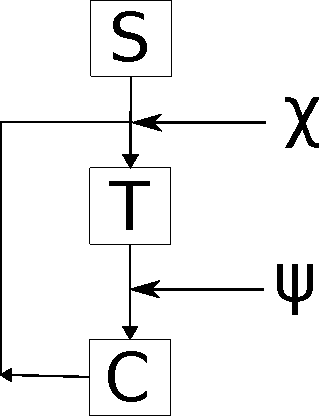
\includegraphics[width=1.25in]{../document/chapters/random_walk_process_derivation/random_walk_process.pdf}
    \end{center}
  \end{figure}

  %% \begin{textblock}{20}(80,50)
  %%   \begin{align}
  %%     R & = \langle r \text{ } \varphi \rangle \nonumber \\
  %%     & = \langle r_{\psi} \text{ } \psi \rangle \nonumber \\
  %%     & = \langle r_{\chi} \text{ } \chi \rangle \nonumber
  %%   \end{align}
  %% \end{textblock

\end{frame}

%%----------------------------------------------------------------------------%%
\subsection{The Monte Carlo random walk process for adjoint radiation transport}
%%----------------------------------------------------------------------------%%
\begin{frame}{The Adjoint Transport Equation Forcing Function}

  \begin{itemize}
    \item A material response can be calculated using the flux and a material
      response function $r(\vec{r},E,\hat{\Omega})$
  \end{itemize}
  \begin{equation*}
    R = \langle \varphi r \rangle
  \end{equation*}
  
  \begin{itemize}
    \item The flux is characterized by the transport equation 
  \end{itemize}
  \begin{equation*}
    H_B \cdot \varphi(\vec{r},E,\hat{\Omega}) = S(\vec{r},E,\hat{\Omega})
  \end{equation*}
  
  \begin{itemize}
    \item The adjoint operator is defined by the following relationship:
  \end{itemize}
  \begin{equation*}
    \langle \varphi^{\dagger}H_B \cdot \varphi \rangle = 
    \langle \varphi H_B^{\dagger} \cdot \varphi^{\dagger} \rangle
  \end{equation*}
  
  \begin{itemize}
    \item Want to calculate the same material response
  \end{itemize}
  \medskip
  \begin{equation*}
    R = \langle \varphi r \rangle 
    = \langle \varphi H_B^{\dagger} \cdot \varphi^{\dagger} \rangle 
    = \langle \varphi^{\dagger}H_B \cdot \varphi \rangle
    = \langle \varphi^{\dagger} S \rangle \nonumber
  \end{equation*}

  \begin{itemize}
    \item The forcing function for the adjoint transport equation must be
      the material response function
  \end{itemize}

\end{frame}

%%----------------------------------------------------------------------------%%
\begin{frame}{The Adjoint Transport Equation}

  \begin{itemize}
    \item Using the definition of the adjoint operator, the adjoint transport 
      equation can be derived
  \end{itemize}
  
  \begin{equation*}
    \begin{split}
      -\hat{\Omega} &\cdot \vec{\bigtriangledown} 
      \varphi^{\dagger}(\vec{r},E,\hat{\Omega})
      + \Sigma_T(\vec{r},E) \varphi^{\dagger}(\vec{r},E,\hat{\Omega}) = \\
      & \quad r(\vec{r},E,\hat{\Omega}) +
      \int\int \Sigma_T(\vec{r},E \to E^{'},\hat{\Omega} \to \hat{\Omega}^{'})
      \varphi^{\dagger}(\vec{r},E^{'},\hat{\Omega}^{'}) dE^{'}d\hat{\Omega}^{'}
    \end{split}
  \end{equation*}

  \medskip

  \begin{itemize}
    \item The right side of this equation is called the adjoint emission density
  \end{itemize}
  \begin{equation*}
    \theta^{\dagger}(\vec{r},E,\hat{\Omega}) = r(\vec{r},E,\hat{\Omega}) +
    \int\int \Sigma_T(\vec{r},E \to E^{'},\hat{\Omega} \to \hat{\Omega}^{'})
    \varphi^{\dagger}(\vec{r},E^{'},\hat{\Omega}^{'}) dE^{'}d\hat{\Omega}^{'}
  \end{equation*}

  \begin{itemize}
    \item This equation must be converted to a FIESK to derive
      a Monte Carlo random walk process for adjoint radiation transport
  \end{itemize}
      
\end{frame}

%%----------------------------------------------------------------------------%%
\begin{frame}{The Adjoint Transport Equation in Integral Form}

  \begin{itemize}
    \item The method of characteristics is used to convert the adjoint transport
      equation to an ordinary differential equation (ODE)
      \medskip
    \item Subsequent solution of this ODE results in the integral adjoint 
      transport equation
  \end{itemize}
  \begin{align}
    \varphi^{\dagger}(\vec{r},E,\hat{\Omega}) & = 
    \int_0^{\infty} \theta^{\dagger}(\vec{r} + R\hat{\Omega},E,\hat{\Omega})
    exp\left[-\int_0^R \Sigma_T(\vec{r}+R^{'}\hat{\Omega},E)dR^{'} \right] dR
    \nonumber \\
    & = \int \theta^{\dagger}(\vec{r}^{'},E,\hat{\Omega}) 
    \tau^{\dagger}(\vec{r}^{'},\vec{r},E,\hat{\Omega}) dV^{'} \nonumber
  \end{align}

  \begin{itemize}
    \item The function $\tau^{\dagger}(\vec{r}^{'},\vec{r},E,\hat{\Omega})$ allows
      the line integral to be expressed as a volume integral
  \end{itemize}
  \begin{equation*}
    \tau^{\dagger}(\vec{r}^{'},\vec{r},E,\hat{\Omega}) = 
    \exp{\left[-\int_0^{|\vec{r}^{'} - \vec{r}|} 
        \Sigma_T(\vec{r}+R^{'}\hat{\Omega},E)dR^{'} \right]}
    \frac{\delta \left(\hat{\Omega} - \left[\frac{\vec{r}^{'} - \vec{r}}
        {|\vec{r}^{'} - \vec{r}|}\right]\right)}
         {|\vec{r}^{'} - \vec{r}|^2}
  \end{equation*}

\end{frame}

%%----------------------------------------------------------------------------%%
\begin{frame}{The Adjoint Emission Density FIESK}

  \begin{itemize}
    \item To construct the adjoint emission density FIESK, the integral 
      adjoint transport equation is substituted into the equation for
      the adjoint emission density:
  \end{itemize}
  \begin{align}
    \theta^{\dagger}(\vec{r},E,\hat{\Omega}) & = r(\vec{r},E,\hat{\Omega}) +
    \int\int \Sigma_T(\vec{r},E \to E^{'},\hat{\Omega} \to \hat{\Omega}^{'})
    \nonumber \\
    & \qquad \qquad \qquad \qquad \cdot
    \int \theta^{\dagger}(\vec{r}^{'},E^{'},\hat{\Omega}^{'}) 
    \tau^{\dagger}(\vec{r}^{'},\vec{r},E^{'},\hat{\Omega}^{'}) 
    dV^{'} dE^{'} d\hat{\Omega}^{'} \nonumber \\
    & = r(\vec{r},E,\hat{\Omega}) +
    \int\int\int M^{\dagger}(\vec{r}^{'} \to \vec{r},E^{'} \to E,
        \hat{\Omega}^{'} \to \hat{\Omega}) \nonumber \\
         & \qquad \qquad \qquad \qquad \qquad \cdot
         \theta^{\dagger}(\vec{r}^{'},E^{'},\hat{\Omega}^{'}) 
         dV^{'} dE^{'} d\hat{\Omega}^{'} \nonumber
  \end{align}

  \begin{itemize}
    \item The kernel of the adjoint emission density FIESK is
      \begin{align}
        M^{\dagger}(y \to x) & = M^{\dagger}(\vec{r}^{'} \to \vec{r},E^{'} \to E,
        \hat{\Omega}^{'} \to \hat{\Omega}) \nonumber \\
        & = \Sigma_T(\vec{r},E \to E^{'},\hat{\Omega} \to \hat{\Omega}^{'})
        \tau^{\dagger}(\vec{r}^{'},\vec{r},E^{'},\hat{\Omega}^{'}) \nonumber
      \end{align}
    \item This kernel can be simplified by introducing two new kernels
  \end{itemize}

\end{frame}

%%----------------------------------------------------------------------------%%
\begin{frame}{The Adjoint Transport Kernel}

  \begin{align}
    T^{\dagger}(\vec{r}^{'} \to &\vec{r},E,\hat{\Omega}) = 
    \Sigma_T(\vec{r},E) \tau^{\dagger}(\vec{r}^{'},\vec{r},E,\hat{\Omega})
    \nonumber \\
    & = \Sigma_T(\vec{r},E) \exp{\left[-\int_0^{|\vec{r}^{'} - \vec{r}|} 
        \Sigma_T(\vec{r}+R^{'}\hat{\Omega},E)dR^{'} \right]} %%\nonumber \\
    %%& \qquad \qquad \qquad \qquad \cdot
    \frac{\delta \left(\hat{\Omega} - \left[\frac{\vec{r}^{'} - \vec{r}}
        {|\vec{r}^{'} - \vec{r}|}\right]\right)}
         {|\vec{r}^{'} - \vec{r}|^2} \nonumber
  \end{align}

  \begin{itemize}
    \item Describes the movement of adjoint particles through space
      \medskip
    \item Quantity $T^{\dagger}(\vec{r}^{'} \to \vec{r},E,\hat{\Omega})dV$ is 
      probability that an adjoint particle at $\vec{r}^{'}$ with energy $E$ and 
      direction $\hat{\Omega}$ will have next collision in volume element $dV$ 
      at $\vec{r}$
      \medskip
    \item The factor $\Sigma_T(\vec{r},E)$ prevents new positions $\vec{r}$ 
      from begin sampled in a vacuum
  \end{itemize}

\end{frame}

%%----------------------------------------------------------------------------%%
\begin{frame}{The Adjoint Collision Kernel}

  \begin{align}
    C^{\dagger}(\vec{r},E^{'} \to E,\hat{\Omega}^{'} \to \hat{\Omega}) & = 
    \frac{\Sigma_T(\vec{r},E \to E^{'},\hat{\Omega} \to \hat{\Omega}^{'})}
         {\int\int \Sigma_T(\vec{r},E \to E^{'},\hat{\Omega} \to \hat{\Omega}^{'})
           dE d\hat{\Omega}} \nonumber \\
         & = \frac{\Sigma_T(\vec{r},E \to E^{'},\hat{\Omega} \to \hat{\Omega}^{'})}
         {\Sigma^{\dagger}(\vec{r},E^{'})} \nonumber
  \end{align}

  \begin{itemize}
    \item Describes the movement of adjoint particles through energy and 
      direction
      \medskip
    \item Not immediately clear what this kernel should integrate to - force it
      to integrate to unity for simplicity
      \medskip
    \item Normalization factor is referred to simply as the total macroscopic 
      adjoint cross section
      \medskip
    \item Expansion of this kernel is necessary to derive a sampling procedure
  \end{itemize}

\end{frame}

%%----------------------------------------------------------------------------%%
\begin{frame}{The Expanded Adjoint Collision Kernel}
  
  \begin{align}
    C^{\dagger}(\vec{r},&E^{'} \to E,\hat{\Omega}^{'} \to \hat{\Omega}) =
    \frac{\Sigma_T(\vec{r},E \to E^{'},\hat{\Omega} \to \hat{\Omega}^{'})}
         {\Sigma^{\dagger}(\vec{r},E^{'})} \nonumber \\
         & = \sum_j 
         \frac{\Sigma_{j}(\vec{r},E)c_j(\vec{r},E)
           f_j(E \to E^{'},\hat{\Omega} \to \hat{\Omega}^{'})}
              {\Sigma^{\dagger}(\vec{r},E^{'})} \nonumber \\
              & = \sum_A \frac{\Sigma_A^{\dagger}(\vec{r},E^{'})}
              {\Sigma^{\dagger}(\vec{r},E^{'})}
              \sum_j \frac{\sigma_{A,j}^{\dagger}(E^{'})}{\sigma_A^{\dagger}(E^{'})}
              \frac{\sigma_{A,j}(E) c_{A,j}(E) 
                p_{A,j}(E \to E^{'},\hat{\Omega} \to \hat{\Omega}^{'})}
                   {\sigma_{A,j}^{\dagger}(E^{'})} \nonumber
  \end{align}

  \medskip

  \begin{itemize}
    \item Through expansion the definition of the adjoint cross section also 
      becomes clear
  \end{itemize}
  \begin{equation*}
    \sigma_{A,j}^{\dagger}(E^{'}) = \int\int
    \sigma_{A,j}(E)c_{A,j}(E) 
    p_{A,j}(E \to E^{'},\hat{\Omega} \to \hat{\Omega}^{'}) dE d\hat{\Omega}
  \end{equation*}
  \begin{equation*}
    p_{A,j}^{\dagger}(E^{'} \to E,\hat{\Omega}^{'} \to \hat{\Omega}) = 
    \frac{\sigma_{A,j}(E)c_{A,j}(E) 
      p_{A,j}(E \to E^{'},\hat{\Omega} \to \hat{\Omega}^{'})}
         {\sigma_{A,j}^{\dagger}(E^{'})}
  \end{equation*}
      
\end{frame}

%%----------------------------------------------------------------------------%%
\begin{frame}{The Adjoint Emission Density FIESK Revisited}
  
  \begin{itemize}
    \item The state transition kernel for the adjoint emission density FIESK 
      can be simplified using the previous two kernels
  \end{itemize}
  \begin{align}
    M^{\dagger}(&y \to x) = M^{\dagger}(\vec{r}^{'} \to \vec{r},E^{'} \to E,
    \hat{\Omega}^{'} \to \hat{\Omega}) \nonumber \\
    & = \Sigma_T(\vec{r},E \to E^{'},\hat{\Omega} \to \hat{\Omega}^{'})
    \tau^{\dagger}(\vec{r}^{'},\vec{r},E^{'},\hat{\Omega}^{'}) \nonumber \\
    & = \left[
      \frac{\Sigma_T(\vec{r},E \to E^{'},\hat{\Omega} \to \hat{\Omega}^{'})}
           {\Sigma^{\dagger}(\vec{r},E^{'})}\right]
    \left[\frac{\Sigma^{\dagger}(\vec{r},E^{'})}{\Sigma_T(\vec{r},E^{'})}\right]
    \left[\Sigma_T(\vec{r},E^{'})
    \tau^{\dagger}(\vec{r}^{'},\vec{r},E^{'},\hat{\Omega}^{'})\right] 
    \nonumber \\
    & = C^{\dagger}(\vec{r},E^{'} \to E,\hat{\Omega}^{'} \to \hat{\Omega})
    P^{\dagger}(\vec{r},E^{'})
    T^{\dagger}(\vec{r}^{'} \to \vec{r},E^{'},\hat{\Omega}^{'}) \nonumber
  \end{align}

  \begin{itemize}
    \item This kernel also contains a factor $P^{\dagger}(\vec{r},E^{'})$ called 
      the adjoint weight factor
      \medskip
    \item This factor is bounded in the interval (0,$\infty$).
  \end{itemize}

\end{frame}

%%----------------------------------------------------------------------------%%
\begin{frame}{The Adjoint Collision Density FIESK}

  \begin{itemize}
    \item The adjoint collision density and emission density are directly
      related
      \begin{equation*}
        \xi^{\dagger}(\vec{r},E,\hat{\Omega}) =
        \int T^{\dagger}(\vec{r}^{'} \to \vec{r},E,\hat{\Omega})
        \theta^{\dagger}(\vec{r}^{'},E,\hat{\Omega}) dV^{'}
      \end{equation*}
    \item The adjoint collision density FIESK is therefore
  \end{itemize}
  \begin{align}
    \xi^{\dagger}(\vec{r},E,\hat{\Omega}) & = \int r(\vec{r}^{'},E,\hat{\Omega})
    T^{\dagger}(\vec{r}^{'} \to \vec{r},E,\hat{\Omega}) dV^{'} + \nonumber \\
    &\quad \int\int\int N^{\dagger}(\vec{r}^{'} \to \vec{r},E^{'} \to E,
    \hat{\Omega}^{'} \to \hat{\Omega}) 
    \xi^{\dagger}(\vec{r}^{'},E^{'},\hat{\Omega}^{'})
    dE^{'}d\hat{\Omega}^{'}dV^{'} \nonumber
  \end{align}
  
  \begin{itemize}
    \item The state transition kernel for this FIESK is
  \end{itemize}
  \begin{align}
    N^{\dagger}(y \to x) & =
    N^{\dagger}(\vec{r}^{'} \to \vec{r},E^{'} \to E,\hat{\Omega}^{'} \to \hat{\Omega})
    \nonumber \\
    & = T^{\dagger}(\vec{r}^{'} \to \vec{r},E,\hat{\Omega})
    C^{\dagger}(\vec{r}^{'},E^{'} \to E,\hat{\Omega}^{'} \to \hat{\Omega})
    P^{\dagger}(\vec{r}^{'},E^{'}) \nonumber
  \end{align}
  
\end{frame}

%%----------------------------------------------------------------------------%%
\begin{frame}{The Monte Carlo Random Walk Process}
  \begin{itemize}
    \item From the adjoint emission density FIESK and adjoint collision 
      density FIESK, the random walk process can be determined
  \end{itemize}
  \begin{equation*}
    \theta^{\dagger}(x)\text{ Random Walk:}
    \begin{cases}
      p^1(x) & = \frac{a(x)}{\int a(x)dx} \\
      p(y \to x) & = \frac{M^{\dagger}(y \to x)}{\overline{P}^{\dagger}(y)} \\
      p(x) & = 0
    \end{cases}
  \end{equation*}
  \medskip
  \begin{equation*}
    \xi^{\dagger}(x)\text{ Random Walk:}
    \begin{cases}
      p^1(x) & = \frac{S_c^{\dagger}(x)}{\int S_c^{\dagger}(x)dx} \\
      p(y \to x) & = \frac{N^{\dagger}(y \to x)}{P^{\dagger}(y)} \\
      p(x) & = 0
    \end{cases}
  \end{equation*}

  \begin{itemize}
    \item There is no absorption reaction for adjoint radiation
      \smallskip
      \begin{itemize}
        \item Due to the adjoint cross section definition
      \end{itemize}
      \medskip
    \item Russian roulette must be used to end random walks
      \medskip
    \item Both processes can be combined into a single process
  \end{itemize}

\end{frame}

%%----------------------------------------------------------------------------%%
\begin{frame}{The Combined Monte Carlo Adjoint Process}

  \begin{itemize}
    \item The kernels $M^{\dagger}(y \to x)$ and $N^{\dagger}(y \to x)$ only differ
      in the order of the adjoint collision kernel, adjoint transport kernel
      and adjoint weight factor
      \medskip
    \item Both densities can therefore be estimated during the same process
  \end{itemize}
  
  \begin{figure}[h!]
    \begin{center}
      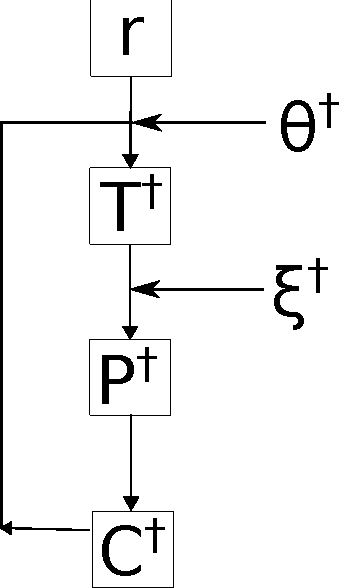
\includegraphics[width=1.0in]{figures/adjoint_random_walk_process.pdf}
    \end{center}
  \end{figure}

\end{frame}

%%----------------------------------------------------------------------------%%
\section{Adjoint Photon Cross Sections}
%%----------------------------------------------------------------------------%%
\subsection{Adjoint photon incoherent scattering}
%%----------------------------------------------------------------------------%%
\begin{frame}{The Adjoint Incoherent Scattering Cross Section}
  
  \begin{itemize}
    \item Use the definition of the adjoint double differential transfer 
      probability to construct this cross section:
  \end{itemize}
  \begin{align}
    p_{i.s.}^{\dagger}(E^{'} \to E, \hat{\Omega}^{'} \to \hat{\Omega}) & =
    \frac{\sigma_{i.s.}(E)c_{i.s.}(E)
      p_{i.s.}(E \to E^{'},\hat{\Omega} \to \hat{\Omega}^{'})}
         {\sigma_{i.s.}^{\dagger}(E^{'})} \nonumber \\
         \sigma_{i.s.}^{\dagger}(E^{'})
         p_{i.s.}^{\dagger}(E^{'} \to E, \hat{\Omega}^{'} \to \hat{\Omega}) & = 
         \sigma_{i.s.}(E)p_{i.s.}(E \to E^{'},\hat{\Omega} \to \hat{\Omega}^{'})
         \nonumber \\ \medskip \nonumber \\
         \sigma_{i.s.}^{\dagger}(E^{'} \to E, \hat{\Omega}^{'} \to \hat{\Omega}) & = 
         \sigma_{i.s.}(E \to E^{'},\hat{\Omega} \to \hat{\Omega}^{'}) \nonumber
  \end{align}

  \begin{itemize}
    \item Both the forward and adjoint cross sections are only dependent on the 
      angle between the initial and final directions:
  \end{itemize}
  \begin{align}
    \sigma_{i.s}^{\dagger}(E^{'} \to E, \hat{\Omega}^{'} \cdot \hat{\Omega}) & = 
    \sigma_{i.s.}(E \to E^{'},\hat{\Omega} \cdot \hat{\Omega}^{'}) \nonumber \\
    \sigma_{i.s}^{\dagger}(E^{'} \to E, \mu) & = 
    \sigma_{i.s.}(E \to E^{'}, \mu) \nonumber
  \end{align}

\end{frame}

%%----------------------------------------------------------------------------%%
\begin{frame}{The Adjoint Incoherent Scattering Cross Section}

  \begin{itemize}
    \item The double differential incoherent scattering cross section is the
      following, where $S(y,Z)$ is the scattering function:
  \end{itemize}
  \begin{align}
    \sigma_{i.s.}(E^{'} \to E, \mu) & = 
    \frac{d^2\sigma_{i.s.}(E^{'},E,\mu,Z)}{dEd\mu} \nonumber \\
    & =  \frac{\pi r_e^2}{m_ec^2 \alpha^{'2}}
    \left[\frac{\alpha}{\alpha^{'}} + \frac{\alpha^{'}}{\alpha} - 
      1 + \mu^2\right] S\left(y(\alpha^{'},\mu),Z\right) \nonumber \\
    & \qquad \qquad \qquad \cdot \delta\left(\mu - \left[1-\frac{1}{\alpha} + 
      \frac{1}{\alpha^{'}}\right]\right) \nonumber
  \end{align}

  \begin{itemize}
    \item The adjoint double differential incoherent scattering cross section
      is therefore
  \end{itemize}
   \begin{align}
    \sigma_{i.s.}^{\dagger}(E^{'} \to E, \mu)  & =  
    \frac{\pi r_e^2}{m_ec^2 \alpha^{2}}
    \left[\frac{\alpha^{'}}{\alpha} + \frac{\alpha}{\alpha^{'}} - 
      1 + \mu^2\right] S\Big(y(\alpha,\mu),Z\Big) \nonumber \\
    & \qquad \qquad \qquad \cdot \delta\left(\mu - \left[1-\frac{1}{\alpha^{'}} 
      + \frac{1}{\alpha}\right]\right) \nonumber
  \end{align}

\end{frame}

%%----------------------------------------------------------------------------%%
\begin{frame}{The Integrated Adjoint Incoherent Scattering Cross Section}

  \begin{itemize}
    \item Limits of integration must be determined to compute the 
      integrated adjoint incoherent cross section
      \medskip
    \item Use the kinematic equation for the adjoint process
  \end{itemize}
  \begin{equation*}
    E = \frac{E^{'}}{1-\alpha^{'}(1-\mu)}
  \end{equation*}
  \begin{align}
    \mu = 1&\text{:} \quad E_{low} = E^{'} \nonumber \\
    \mu = 1 - \frac{1}{\alpha^{'}}&\text{:} \quad E_{high} = \infty \nonumber
  \end{align}
        
  \begin{itemize}
    \item The integrated cross section will be infinite unless a max problem 
      energy is set
  \end{itemize}
  
\end{frame}

%%----------------------------------------------------------------------------%%
\begin{frame}{The Integrated Adjoint Incoherent Scattering Cross Section}

  \begin{figure}[h!]
    \begin{center}
      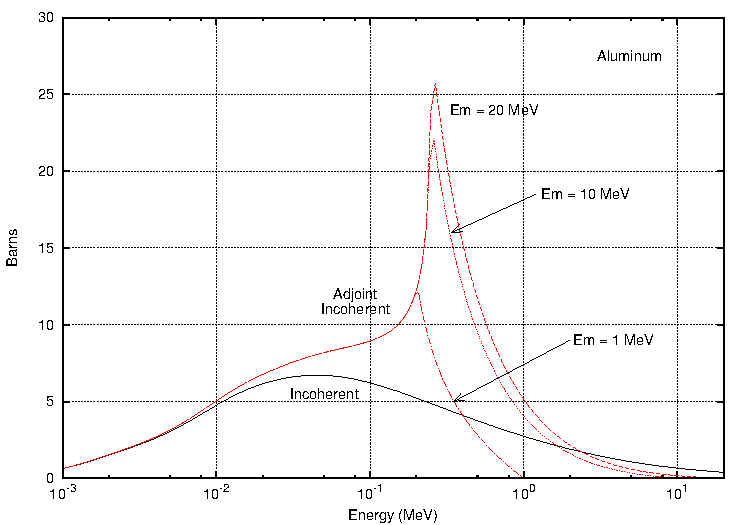
\includegraphics[width=4.0in]{figures/adjoint_and_forward_incoherent_cross_section-13.pdf}
    \end{center}
  \end{figure}

\end{frame}

%%----------------------------------------------------------------------------%%
\subsection{Adjoint photon coherent scattering}
%%----------------------------------------------------------------------------%%
\begin{frame}{The Adjoint Coherent Scattering Cross Section}

  \begin{itemize}
    \item Use the definition of the adjoint double differential cross section
  \end{itemize}
  
  \begin{equation*}
    \sigma_{c.s.}^{\dagger}(E^{'} \to E, \hat{\Omega}^{'} \cdot \hat{\Omega}) =
    \sigma_{c.s.}(E \to E^{'},\hat{\Omega} \cdot \hat{\Omega}^{'})
  \end{equation*}
  
  \bigskip

  \begin{itemize}
  \item In the forward interaction, the energy of the photon does not change: 
  \end{itemize}
  \begin{align}
    \sigma_{c.s.}^{\dagger}(E^{'}, \hat{\Omega}^{'} \cdot \hat{\Omega}) & = 
    \sigma_{c.s.}(E^{'},\hat{\Omega} \cdot \hat{\Omega}^{'}) \nonumber \\
    \frac{d\sigma_{c.s.}^{\dagger}(E^{'}, \mu)}{d\mu} & = 
    \frac{d\sigma_{c.s.}(E^{'}, \mu)}{d\mu} \nonumber
  \end{align}

  \medskip

  \begin{itemize}
    \item Both the forward and adjoint differential coherent scattering cross
      section are therefore the same:
  \end{itemize}
  \begin{align}
    \frac{d\sigma_{c.s.}^{\dagger}(E^{'},\mu,Z)}{d\mu} & = 
    \frac{d\sigma_{c.s.}(E^{'},\mu,Z)}{d\mu} \nonumber \\
    & = \pi r_e^2 (1 + \mu^2)F^2(y,Z) \nonumber
  \end{align}

  \begin{itemize}
    \item F(y,Z) is the atomic form factor
  \end{itemize}

\end{frame}

%%----------------------------------------------------------------------------%%
\subsection{Adjoint photon pair production}
%%----------------------------------------------------------------------------%%
\begin{frame}{The Adjoint Pair Production Cross Section}

  \begin{itemize}
    \item Use the definition of the adjoint double differential cross section
  \end{itemize}
  
  \begin{equation*}
    \sigma_{p.p.}^{\dagger}(E^{'} \to E, \hat{\Omega}^{'} \cdot \hat{\Omega}) =
    2\sigma_{p.p.}(E \to E^{'},\hat{\Omega} \cdot \hat{\Omega}^{'})
  \end{equation*}

  \bigskip

  \begin{itemize}
    \item The simplified double differential pair production cross section is
  \end{itemize}
  \begin{align}
    \sigma_{p.p.}(E^{'} \to E,\mu) & = \frac{d^2\sigma_{p.p.}(E^{'},Z)}{dEd\mu} 
    \nonumber \\
    & = \frac{[\sigma_{p.p.}(E^{'},Z) + \sigma_{t.p.}(E^{'},Z)] 
      \delta(E - m_ec^2)}{2} \nonumber
  \end{align}

  

  \begin{itemize}
    \item The adjoint pair production cross section is therefore
  \end{itemize}
  \begin{align}
    \sigma_{p.p.}^{\dagger}(E^{'} \to E,\mu) & = 
    \frac{d^2\sigma_{p.p.}^{\dagger}(E^{'},E,Z)}{dEd\mu} \nonumber \\
    & = 2\left[\frac{\left[\sigma_{p.p.}(E,Z)+\sigma_{t.p.}(E,Z)\right]
      \delta(E^{'}-m_ec^2)}{2}\right] \nonumber
  \end{align}
  
\end{frame}

%%----------------------------------------------------------------------------%%
\begin{frame}{The Adjoint Pair Production Cross Section}

  \begin{equation*}
    \frac{d^2\sigma_{p.p.}^{\dagger}(E^{'},E,Z)}{dEd\mu} = 
    2\left[\frac{\left[\sigma_{p.p.}(E,Z)+\sigma_{t.p.}(E,Z)\right]
      \delta(E^{'}-m_ec^2)}{2}\right] \nonumber
  \end{equation*}

  \bigskip

  \begin{itemize}
    \item The two annihilation photons are taken into account with the
      factor of 2
      \medskip
    \item Unless the adjoint photon energy is $m_ec^2$ this cross section is 
      zero 
      \medskip
    \item A modification to the adjoint random walk process is made which
      forces adjoint photons to have energy $m_ec^2$
      \medskip
    \item The modification is rather complicated but is fairly computationally
      inexpensive 
  \end{itemize}

\end{frame}  

%%----------------------------------------------------------------------------%%
\begin{frame}{Current Limitation: The Photoelectric Effect}

  \begin{itemize}
    \item \textbf{Problem:} 
      \begin{itemize}
        \item Photoelectric effect occurs when a photon is absorbed by an atom
          \medskip
        \item An electron is ejected leaving an electron shell vacancy
          \medskip
        \item Atomic relaxation occurs to fill the vacancy with x-rays 
          potentially released
          \medskip
        \item Emitted x-rays can be important for certain problems (e.g. 
          brachytherapy seed characterization)
          \medskip
        \item The adjoint process cannot currently take these x-rays into 
          account
          \medskip
      \end{itemize}
      \bigskip
    \item \textbf{Possible Solution:} Compute x-ray production cross sections
      for which equivalent adjoint cross sections can be computed
  \end{itemize}

\end{frame}

%%----------------------------------------------------------------------------%%
\subsection{The adjoint photon weight factor}
%%----------------------------------------------------------------------------%%
\begin{frame}{The Adjoint Photon Weight Factor}

  \begin{itemize}
    \item Important feature of the adjoint process.
      \medskip
    \item Bound to the interval (0,$\infty$) instead of (0,1)
      \medskip
    \item Can negatively effect the statistics of the random walks.
      \medskip
    \item Thorough characterization of its effects must be completed.
      \medskip
  \end{itemize}
  
  \begin{figure}[h!]
    \begin{center}
      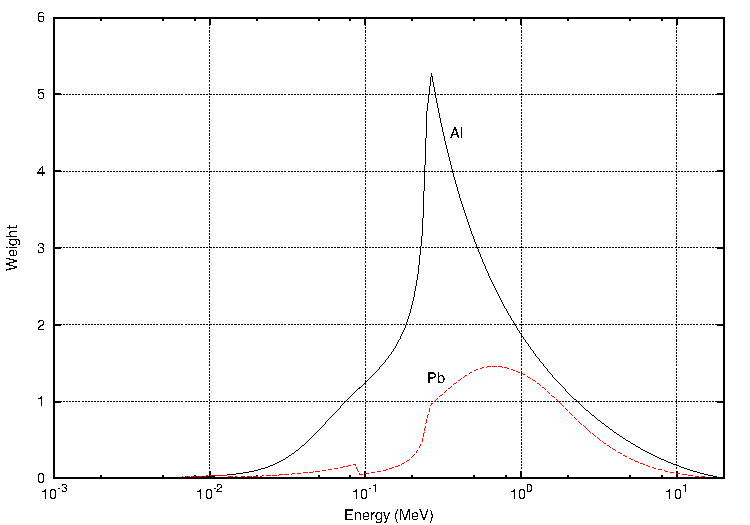
\includegraphics[width=3.0in]{../document/chapters/photon_interactions/adjoint_weight_factor.pdf}
    \end{center}
  \end{figure}

  
\end{frame}

%%----------------------------------------------------------------------------%%
\section{Forward-Adjoint Continuous Energy Monte Carlo (FACEMC) Code}
%%----------------------------------------------------------------------------%%
\subsection{Code overview}
%%----------------------------------------------------------------------------%%
\begin{frame}{FACEMC Code Requirements}


  \begin{itemize}
    \item \textbf{Energy Range:}
      \begin{itemize}
        \item 1 keV - 20 MeV for photons and adjoint photons
        \item $10^{-5}$ eV - 20 MeV for neutrons and adjoint neutrons
          \bigskip
      \end{itemize}
    \item \textbf{Spatial Domain Modeling:} CAD based (primarily)
      \begin{itemize}
        \item Accomplished with the direct accelerated geometry (DAG) package
      \end{itemize}
      \bigskip
    \item \textbf{Variance Reduction:} implicit capture, Russian roulette,
      splitting, forced collisions, weight windows
      \begin{itemize}
        \item Weight windows must be user generated
      \end{itemize}
      \bigskip
    \item \textbf{Parallelism:} domain replication
  \end{itemize}

\end{frame}

%%----------------------------------------------------------------------------%%
%% \begin{frame}{Major Components of FACEMC}
  
%%   \begin{textblock}{20}(20,15)
%%     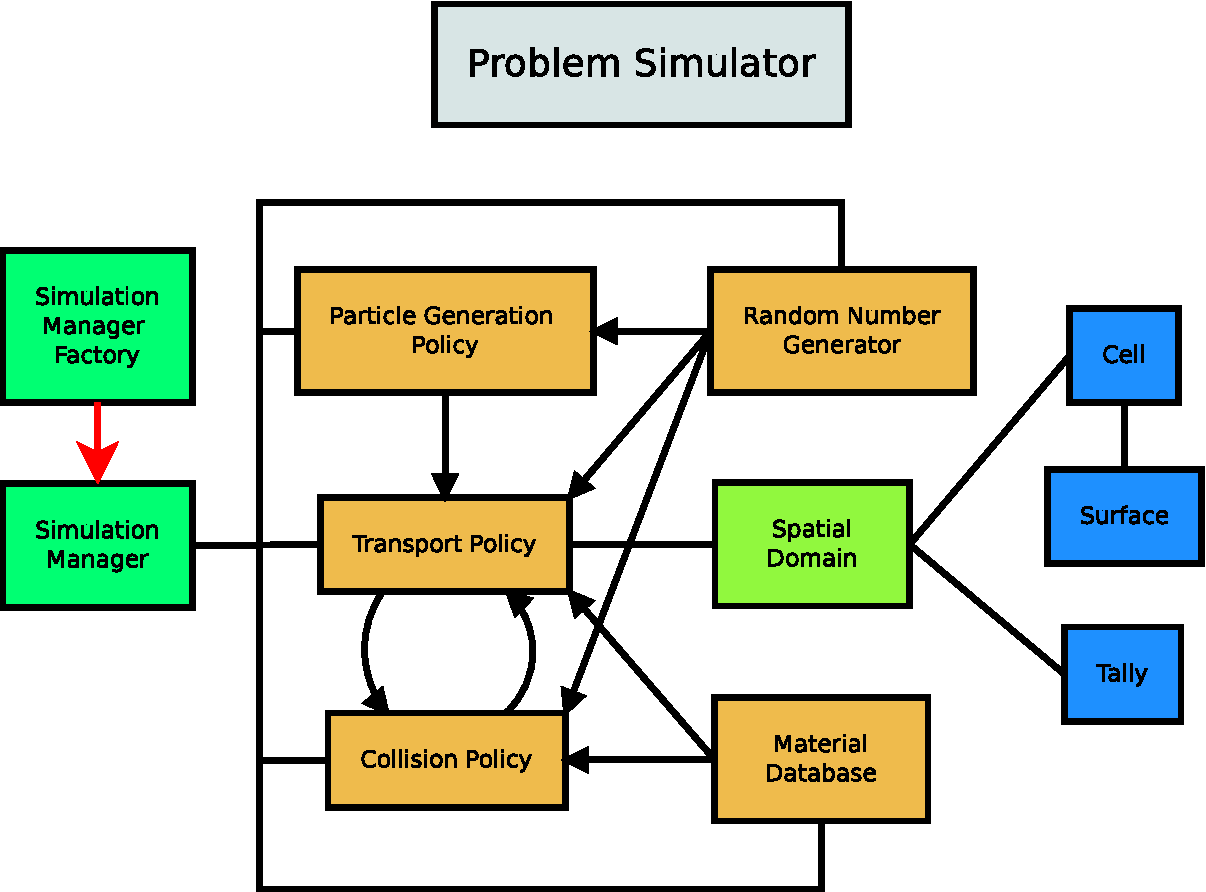
\includegraphics[width=3.5in]{../document/chapters/code_overview/Problem_Simulator.pdf}
%%   \end{textblock}

%%   \begin{textblock}{120}(4,85)
%%     \begin{itemize}
%%       \item FACEMC version 1.0 is currently complete.
%%     \end{itemize}
%%   \end{textblock}

%% \end{frame}

%%----------------------------------------------------------------------------%%
\subsection{Validation plan}
%%----------------------------------------------------------------------------%%
\begin{frame}{FACEMC Validation Plan}

      \begin{enumerate}
        \item \textbf{Benchmarking:} simulation of benchmark test problems for 
          photons and neutrons
          \bigskip
          \bigskip
        \item \textbf{Code-to-Code Comparisons:} calculate integral quantities 
          and spectra and compare against other validated Monte Carlo codes 
          \bigskip
          \bigskip
        \item \textbf{Intra-Code Comparisons:} calculate integral quantities 
          and spectra using FACEMC forward and adjoint simulations
      \end{enumerate}
    
\end{frame}

%%----------------------------------------------------------------------------%%
\begin{frame}{FACEMC Validation Plan: Step 1}

  \begin{textblock}{120}(4,15)
    \begin{itemize}
      \item \textbf{GEANT4 Photon Benchmark Problem:} calculate mass 
        attenuation coefficients and partial interaction coefficients
        \medskip
      \item Results will be compared to NIST values
    \end{itemize}
  \end{textblock}
  
  \begin{textblock}{20}(30,43)
    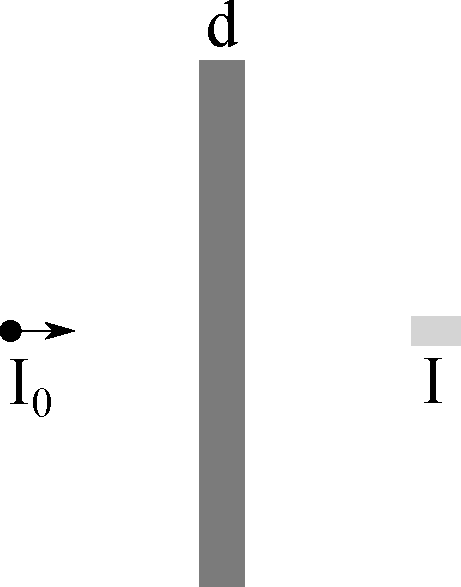
\includegraphics[width=1.0in]{../document/chapters/code_overview/photon_benchmark_problem.pdf}
  \end{textblock}

  \begin{textblock}{20}(65,52)
    \begin{equation*}
      \left(\frac{\mu}{\rho}\right) = -\frac{1}{\rho d}
      \ln{\left(\frac{\text{I}}{\text{I}_0}\right)}
    \end{equation*}
  \end{textblock}

  \begin{textblock}{120}(4,80)
    \begin{itemize}
      \item For neutrons, several experiments from the Shielding Integral
        Benchmark Archive Database (SINBAD) will be modeled
    \end{itemize}
  \end{textblock}

\end{frame}

%%----------------------------------------------------------------------------%%
\begin{frame}{FACEMC Validation Plan: Step 2}
  
  \begin{itemize}
    \item \textbf{Problem Geometry:}
  \end{itemize}
      
  \begin{figure}[h!]
    \begin{center}
      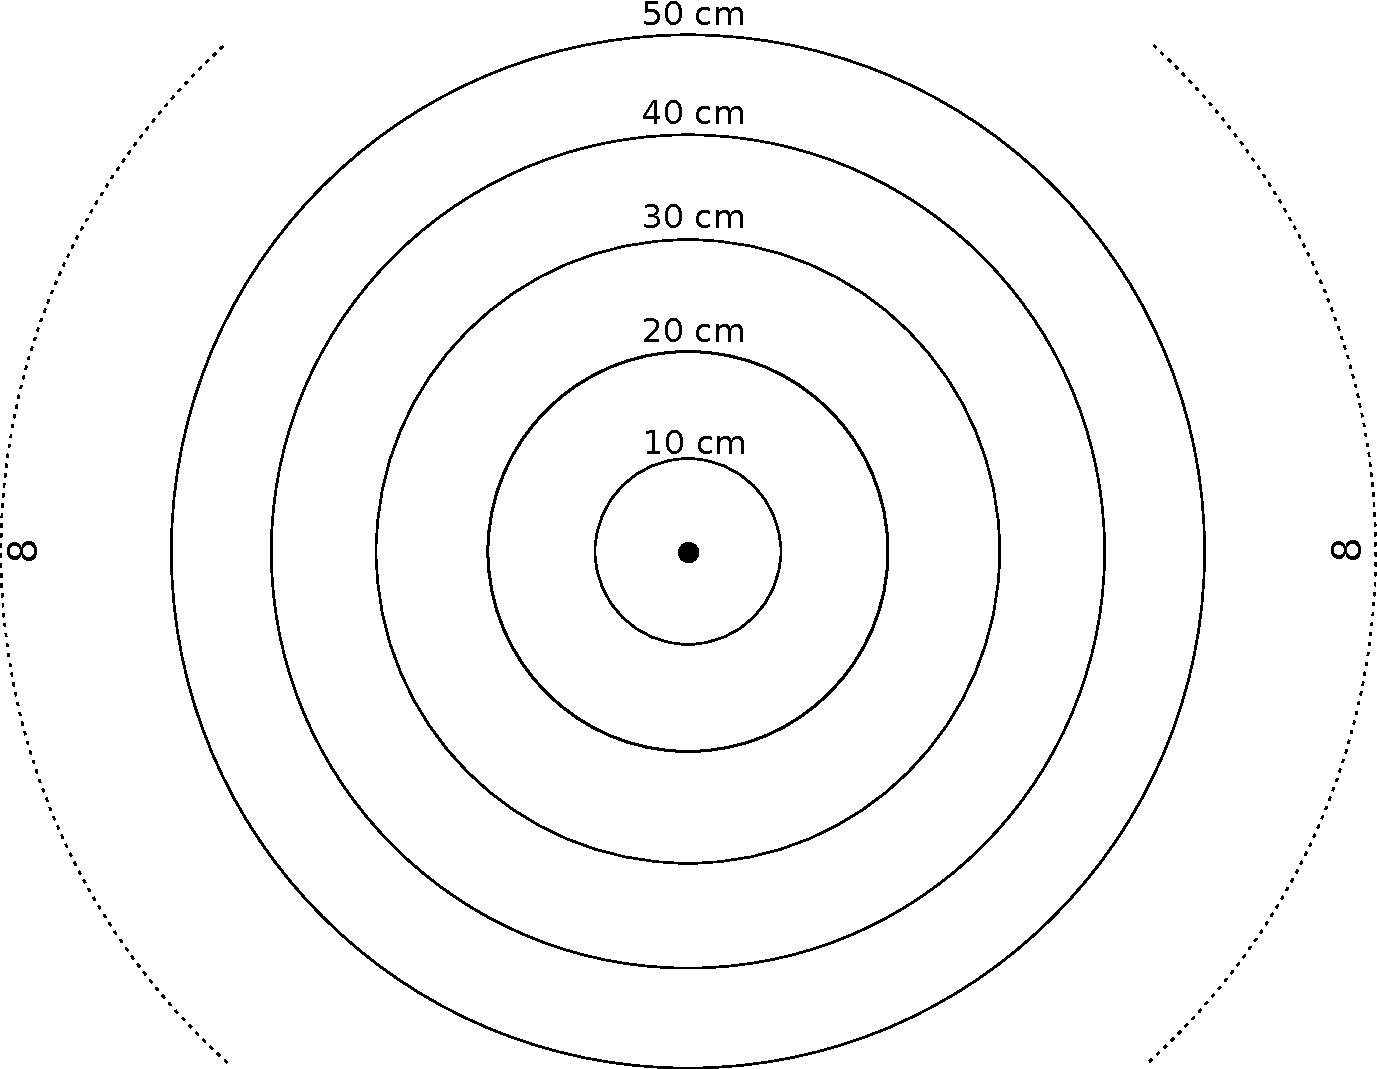
\includegraphics[width=1.7in]{figures/code_comparison_problem.pdf}
    \end{center}
  \end{figure}

  \begin{itemize}
    \item \textbf{Source:}
      \begin{itemize}
        \item isotropic point source with several discrete energies (photons)
        \item isotropic point source with a fission spectrum (neutrons)
      \end{itemize}
      \medskip
    \item \textbf{Quantities:} Flux spectrum and total flux at each spherical 
      surface
      \medskip
    \item \textbf{Comparison Codes:} PENELOPE, MCNP5 and TART2005 
  \end{itemize}
  
\end{frame}

%%----------------------------------------------------------------------------%%
\begin{frame}{FACEMC Validation Plan: Step 3}

  \begin{itemize}
    \item \textbf{Problem Geometry:} same as FACEMC validation plan step 2
      \begin{itemize}
        \item Due to unique symmetry, the adjoint problem can be constructed 
          identically to the forward problem (point source)
      \end{itemize}
      \bigskip
      \bigskip
    \item \textbf{Source:} same as FACEMC validation plan step 2
      \bigskip
      \bigskip
    \item \textbf{Quantities:} Flux spectrum and total flux at each spherical 
      surface

  \end{itemize}    

\end{frame}

%%----------------------------------------------------------------------------%%
\begin{frame}{Preliminary Validation of FACEMC: AMOS Comparison}

  \begin{itemize}
    \item \textbf{Problem Geometry:} simple irradiation facility
      \begin{itemize}
        \item The source is located behind the tungsten alloy collimator.
      \end{itemize}
  \end{itemize}

  \begin{figure}[h!]
    \begin{center}
      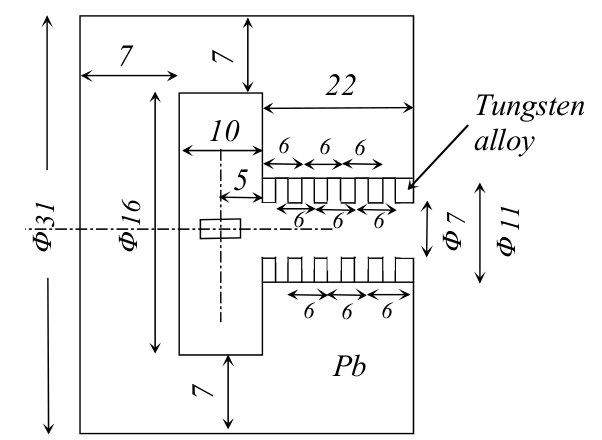
\includegraphics[width=2.3in]{figures/Irradiator_Facility.png}
    \end{center}
  \end{figure}

  \begin{itemize}
    \item \textbf{Source:} isotropically emitting Cs-137 gamma source
      \medskip
    \item \textbf{Quantity:} flux spectrum 50 cm from center of source (on axis)
      \medskip
    \item \textbf{Comparison Code:} AMOS (TU Dresden research code)
  \end{itemize}

\end{frame}

%%----------------------------------------------------------------------------%%
\begin{frame}{AMOS Comparison Results}

  \begin{figure}[h!]
    \begin{center}
      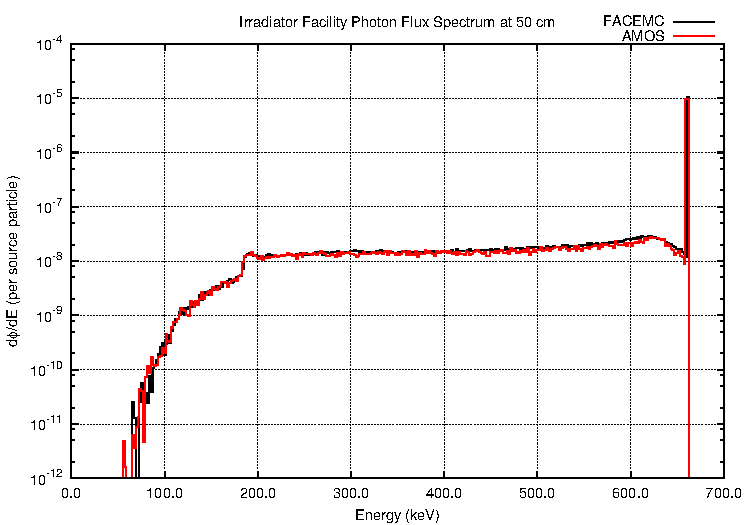
\includegraphics[width=4in]{figures/facemc_amos_irradiator_comp.pdf}
    \end{center}
  \end{figure}

\end{frame}

%%----------------------------------------------------------------------------%%
\begin{frame}{Preliminary Validation of FACEMC: Forward vs. Adjoint}

  \begin{itemize}
    \item \textbf{Problem Geometry:} same as FACEMC validation step 3
    \item \textbf{Source:} isotropic point source emitting at 661.66 keV 
      (80\%) and 321.0 keV (20\%)
    \item \textbf{Material:} water
    \item \textbf{Number of histories:} $10^7$
  \end{itemize}
  
    \begin{table}[ht]
      \centering
      \begin{tabular}{c c c c c c}
        \hline\hline
        Distance & Flux & Relative & Flux & Relative & \% Diff. \\ 
        (cm) & (for. mode) & Error & (adj. mode) & Error &  \\ [0.5ex]
        \hline
        10 & 1.5748e-3 & 0.0007 & 1.5788e-3 & 0.0014 & 0.25 \\
        20 & 4.1291e-4 & 0.0007 & 4.1491e-4 & 0.0018 & 0.48 \\
        30 & 1.4150e-4 & 0.0007 & 1.4235e-4 & 0.0022 & 0.60 \\
        40 & 5.2255e-5 & 0.0011 & 5.2322e-5 & 0.0027 & 0.13 \\
        50 & 1.9963e-5 & 0.0014 & 2.0030e-5 & 0.0033 & 0.34 \\ [1ex]
        \hline
      \end{tabular}
      \label{table:val_plan_s3_c0_flux_water}
    \end{table}   

\end{frame}

%%----------------------------------------------------------------------------%%
\begin{frame}{Forward vs. Adjoint Spectrum Results}
  
  \begin{figure}[h!]
     \begin{center}
       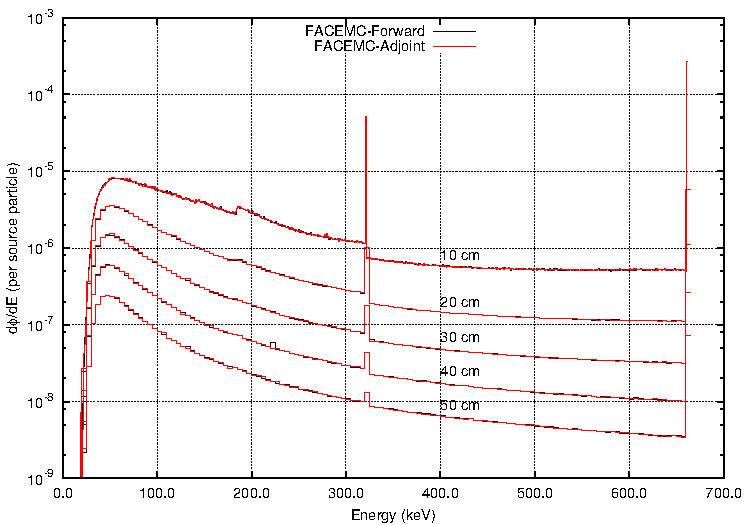
\includegraphics[width=4in]{../document/chapters/code_overview/photon_spectrum_validation_comparison.pdf}
     \end{center}
   \end{figure}

\end{frame}

%%----------------------------------------------------------------------------%%
\section{Future Work}
%%----------------------------------------------------------------------------%%
\begin{frame}{Future work on FACEMC: Development}

  \begin{enumerate}
    \item Solve the low energy x-ray emission problem for adjoint photons
      %% \smallskip
      %% \begin{itemize}
      %%   \item Solution proposed
      %% \end{itemize}
      \medskip
    \item Complete background work on neutron and adjoint neutron transport 
      cross sections and sampling techniques
      %% \smallskip
      %% \begin{itemize}
      %%   \item Adjoint cross section generation generally no more challenging
      %%     than for photons, more numerically intensive
      %% \end{itemize}
      \medskip
    \item Complete coding of the second version of all major FACEMC 
      components 
      %% \smallskip
      %% \begin{itemize}
      %%   \item Based on experience from version 1.0, this will take anywhere
      %%     from 3 to 6 months to complete
      %% \end{itemize}
      \medskip
    \item Complete the computation of adjoint neutron cross sections and 
      storage in an HDF5 format library
      \medskip
    \item Complete the FACEMC validation plan
      \medskip
    \item Characterize the effect of the adjoint weight factor on the 
      variance of the adjoint process
  \end{enumerate}

\end{frame}

%%----------------------------------------------------------------------------%%
\begin{frame}{Future work on FACEMC: Challenge Problems}
  
    \begin{enumerate}
      \item Calculate the adjoint data required for brachytherapy treatment 
        planning optimization using data from a patient
        \bigskip
      \item Calculate the adjoint data required for external beam treatment 
        planning using a standard phantom
        \bigskip
      \item Run a full scale shutdown dose calculation for a fusion device using
        the R2SA method
        \bigskip
      \item Run a fusion shielding problem using the adjoint neutron transport 
        capabilities of FACEMC
    \end{enumerate}
  
\end{frame}

%%----------------------------------------------------------------------------%%
\begin{frame}{Acknowledgments}

  Thanks to...
  
  \begin{itemize}
    \item Douglass Henderson
    \item Bruce Thomadsen
    \item TU Dresden
    \item The NRC
  \end{itemize}

  \medskip \medskip \medskip \medskip \medskip \medskip \medskip

  \begin{beamerboxesrounded}[upper=boxheadcolor,lower=boxbodycolor,shadow=true]{Support}
    This work was performed under appointment to the Nuclear Regulatory
    Commission Fellowship program at the University of Wisconsin - Madison
    Department of Engineering Physics.
  \end{beamerboxesrounded}

\end{frame}

%%----------------------------------------------------------------------------%%

\end{document}

